\section{Computer Science Approach}
\label{sec:ComputerScienceApproach}

The following definitions are adopted from the code:

\begin{lstlisting}[language=C, caption=Data type definitions, label=lst:definitions]
#define FLT float
#define INS int
#define DBL double
#define INT long
#define UCHR unsigned char
#define CHR char
#define UINT unsigned int
#define ULON unsigned long
\end{lstlisting}

\subsection{VTK format}
\label{subsec:VTKformat}

The Visualisation Toolkit \texttt{VTK} \cite{Kit} is an extremely popular open source software for graphic visualisation of scientific data. \texttt{VTK} \texttt{API}s are available in many different programming languages and facilitate the generation of \texttt{VTK} files. Until now, the \texttt{Y} code used the \texttt{C} programming language \texttt{VTK} \texttt{API} to generate simulation output. 

\bigbreak
The required \texttt{VTK} version \texttt{5.8} library dependencies revealed themselves to be outdated and unobtainable. This limited the applicability of the entire \texttt{Y} code to operating systems which support this obsolete version. Specifically, all attempts by the author to obtain such a version for testing were not successful. Rewriting the code using a newer \texttt{VTK} version would only temporarily solve the problem.

\bigbreak
To diversify application to a wider range of operating systems, it was deemed necessary to hard code the output with eschewal of \texttt{VTK} libaries. Aside from the partly ill-documented offical website \cite{Kit}, one of the only few reliable resources available is the \texttt{Earth Models} website by Bunge \cite{Bun09}. In what follows, the aim is to provide the reader with a more detailed and more in-depth description of the \texttt{VTK} format. 

\subsection{VTK legacy file format}
\label{subsec:VTKlegacyfileformat}

The \texttt{VTK} legacy file format is sufficiently documented (see \cite{Kit} for official documentation) and relatively easy to implement. On the downside, it only supports a minimal amount of features and is relatively inflexible. List. \ref{lst:vtklegacy} shows an example \texttt{VTK} legacy file. 

\bigbreak
The header defines \texttt{VTK} version, file name, data encoding (\texttt{ascii} or \texttt{binary}) and dataset type \footnote{here: unstructured grid} \cite{Kit}.

\bigbreak
The data is divided into sections including points, cells, cell types. The section header contains the keyword along with the total amount of entities of the section. The data is written continuously using spaces as separators. \cite{Kit}

\bigbreak
Every section has additional unique formatting rules. The points sections requires an additional data type identifier (here: \lstinline{float}) to correctly identify the coordinates data. \cite{Kit}

\bigbreak
The data in the cells section lists the node numbers of each element, appended to a number identifying the total amount of nodes of the element. \cite{Kit}

\bigbreak
The cell type section identifies the geometric shape of each element, given by an index. Each index is written on a separate line. \cite{Kit}

\subsection{VTK XML file format}
\label{subsec:VTKXMLfileformat}

Compared to \texttt{legacy} files, \texttt{XML} files are much more difficult to implement. An example is given in List. \ref{lst:vtkxmlinline}. 

\bigbreak
The file is structured using nested keyword headers which are enclosed in angle brackets ("<" and ">"), according to \texttt{XML} language. Text indentation is not required but enhances readability.

\bigbreak
Keyword headers are opened using \lstinline[language=XML]{<keyword>} and closed using \lstinline[language=XML]{</keyword>}. Keywords which do not contain any sub-keyword headers are opened and closed in one line using \lstinline[language=XML]{<keyword\>}. Keyword headers usually contain additional mandatory and optional keywords in the format of \lstinline[language=XML]{option="value"} \cite{Kit}.

\bigbreak
The file header specifies versions, \texttt{VTK} file type and \lstinline[language=XML]{byte_order} \footnote{endianess, here: little endian} \cite{Kit}. Big endian byte order was not tested, as such operating systems were not available for testing.

\bigbreak
Depending on the specified \lstinline[language=XML]{VTKFile type}, a unique set of sub-keyword headers is used. For the \lstinline[language=XML]{Unstructured_Grid} \texttt{VTK} file type chosen here, the file content is structured using \lstinline[language=XML]{<Piece>}. Within this header, it is required to specify the number of points and cells (elements) using \lstinline[language=XML]{NumberOfPoints} and \lstinline[language=XML]{NumberOfCells} \cite{Kit}.

\bigbreak
\lstinline{<Piece>} contains definition of \lstinline[language=XML]{<Points>} and \lstinline[language=XML]{<Cells>}, among other optional keyword sub-headers. \lstinline[language=XML]{<Points>} expects exactly one \lstinline[language=XML]{<DataArray>} containing the nodal coordinates. \lstinline[language=XML]{<Cells>} expects one \lstinline[language=XML]{<DataArray>} each for the cell connectivity (node configuration of each cell), the cell offsets (offsets in the cell connectivity list), as well as the cell type (cell shape index, see \cite{Kit}) \cite{Bun09}.

\bigbreak
The data, listed after \lstinline[language=XML]{<DataArray>} includes \lstinline[language=XML]{type} (data type), \lstinline[language=XML]{Name}, \lstinline[language=XML]{NumberOfComponents}, \lstinline[language=XML]{format}, \lstinline[language=XML]{RangeMin} and \lstinline[language=XML]{RangeMax}.

\bigbreak
\lstinline[language=XML]{RangeMin} and \lstinline[language=XML]{RangeMax} indicate the minimal and maximal values of the data and are optional\footnote{confirmed by tests}. Simple array search functions were implemented in order to find the individual values.

\bigbreak
\lstinline{Name} specifies a unique name, enclosed by \texttt{""}, for the data set. The data array contained in \lstinline[language=XML]{<Points>} requires no name. The data arrays enclosed by \lstinline[language=XML]{<Cells>} require fixed names \lstinline[language=XML]{Name="connectivity"}, \lstinline[language=XML]{Name="offsets"} and \lstinline[language=XML]{Name="types"} \cite{Kit}.  

\bigbreak
\lstinline[language=XML]{format} specifies the encoding of the data.

\bigbreak
In the case \lstinline{format="ascii"}, the data is provided in decimal form, delimited by spaces, similar to section \ref{subsec:VTKlegacyfileformat} \cite{Bun09}. Specifying an inappropriate data \lstinline[language=XML]{type} for this format will not leave the data completely unusable, although induced type casting may yield unexpected results. The dependence on spaces as delimiters is highly impractical when transferring files between different operating systems and applications. 

\bigbreak
A more robust option is given by \lstinline{format="binary"}. Characters such as "<" (binary encoding of 0b00111100=d060) may potentially appear in binary encoded data. As these characters compose \texttt{XML} keyword headers, binary encoding is not realizable \cite{Bun09}. Thus, the data is encoded to \texttt{base 64} (\texttt{b64}) (see \ref{subsec:b64encoding}). 

\bigbreak
For \texttt{b64} encoding, a data header needs to be prepended to the data. The data header is always of type \lstinline[language=C]{int32} (data size: 4 bytes) and specifies the data size, i.e. the amount of binary bytes of subsequent data. The data size is not to be confused with the length of the printed \texttt{b64} encoded data string in the output file, which is insignificant for now. The data size rather refers to the size of the binary data array in \lstinline[language=C]{bytes}, stored as specified by the datatype in the header. Specifying a data \lstinline[language=XML]{type} of a different \texttt{byte} size for this format produces errors and renders the data useless.

\bigbreak
As an example, consider a \lstinline[language=C]{float32} array which contains $100$ data values. The corresponding header is given by:

\begin{equation}
\label{eq:b64inlineex}
    h=100\,\frac{32\,{\rm bits}}{8\,{\rm bits}/{\rm byte}}=400\,{\rm bytes}
\end{equation}

\bigbreak
The header then needs to be encoded to b64, separately from the data. The encoded header string is immediately followed by the encoded data string, without any delimiters. Considering the fact that the data header type is fixed, the \texttt{b64} encoded data header string length is always the same. Thus, no additional offset is necessary to specify the positional onset of the data after the data header \cite{Bun09}.

\bigbreak
Instead of supplying the data inline, it is possible to append data once, to an \lstinline{<AppendedData>} section at the end of the file. This is achieved by specifying option \lstinline[language=XML]{format="appended"} for each data array keyword header and providing an \lstinline[language=XML]{offset} each time.

\bigbreak
In doing so, the entire data is provided in a single long \texttt{b64} encoded string, appended to an underscore "\_". Like in the inline format, each encoded data string must be prepended by a \texttt{b64} encoded header, which specifies the size of the following unencoded data section in bytes. The headers and the data sections are encoded separately each, without any delimiters between headers and data sections.

\bigbreak
The offset value provided in each \lstinline[language=XML]{<DataArray>} specifies the amount of bytes of unencoded data after the underscore to the beginning of the corresponding header. The method of evaluation of header offsets is illustrated in Tab. \ref{tab:offset}.

\begin{table*}[t]
  \caption{Breakdown of offset values for an example output file with $642$ points and $1280$ cells. The desired (header) offsets are given in column $2$.}
  \begin{tabular}{@{}llllllll@{}}
    Name & header offset & data offset & data size & data type size & values & components & points/cells \\\midrule
    Points & 0 & 4 & 15408 & 8 & 1926 & 3 & 642\\
    Connectivity & 15412 & 15416 & 15360 & 4 & 3840 & 3 & 1280\\
    Offsets & 30776 & 30780 & 5120 & 4 & 1280 & 1 & 1280\\
    Types & 35900 & 35904 & 1280 & 1 & 1280 & 1 & 1280\\
    Points s & 37184 & 37188 & 5136 & 8 & 642 & 1 & 642\\
    Points v & 42324 & 42328 & 15408 & 8 & 1926 & 3 & 642\\
    Points n & 57736 & 57740 & 15408 & 8 & 1926 & 3 & 642\\
    Density & 73148 & 73152 & 5136 & 8 & 642 & 1 & 642\\\bottomrule
  \end{tabular}
  \label{tab:offset}
\end{table*}

\bigbreak
In Tab. \ref{tab:offset}, the header offset of the first header is always $0$. As the unencoded header is always an \lstinline[language=C]{int32} of size $4\,{\rm bytes}$, the first data offset is $4$. For a data array with $1926$ values and data type size $8\,{\rm bytes}$ (e.g. \lstinline[language=C]{float64}), the data size in \lstinline[language=C]{bytes} amounts to $1926\cdot8\,{\rm bytes}=15408{\rm bytes}$. The number of values is comprised by the number of components and the number of points, i.e. $3\cdot642=1926$. The next header offset is evaluated by adding the data size to the data offset, i.e. $4+15408=15412$. The remaining offset values are evaluated accordingly.

\subsection{Base 64 encoding}
\label{subsec:b64encoding}

%\begin{figure}
%\begin{tikzpicture}
% \draw (0,0) node[anchor=north] {float* array}
% \draw (2,0) node[anchor=north] {float}
% \draw (4,0) node[anchor=north] {float byte}
%\node [rectangle split,rectangle split parts=36, rectangle split vertical,draw ] %at (0,0);
%\node [rectangle split,rectangle split parts=32, rectangle split vertical,draw ] %at (0,0);
%\node [rectangle split,rectangle split parts=32, rectangle split vertical,draw ] %at (2,0);
%\node [rectangle split,rectangle split parts=8, rectangle split vertical,draw ] %at (2,0);
%\node [rectangle split,rectangle split parts=8, rectangle split vertical,draw ] %at (2,-1);
%\node [rectangle split,rectangle split parts=8, rectangle split vertical,draw ] %at (2,-2);
%\node [rectangle split,rectangle split parts=8, rectangle split vertical,draw ] %at (2,-3);
%\end{tikzpicture}
%\caption{Data segmentation of a \lstinline{float*} array. Each rectangle %represents one bit in memory.}
%\label{fig:segmentation}
%\end{figure}

The output data consists of one- and two-dimensional \lstinline{int} and \lstinline{float} arrays containing nodal properties, elemental properties and flags. The computer stores the data in binary form, according to byte order (endianess) of the operating system at hand.

\bigbreak
\lstinline{float} numbers are usually stored in \texttt{IEEE-754} format \cite{Asp14}. As the numbers are stored internally, the exact manner of storage is theoretically not significant as long as the position (the significance) of the bits in binary-stored \lstinline{float} is not being violated.   

\bigbreak
As the base64 encoding function takes in a contiguous \lstinline{CHR*} array, the data needs to be segmented into bytes. For the \lstinline{INS} data header, this simply involves conversion from a 4-byte \lstinline{int32} to 4 \lstinline{CHR} bytes. The segmentation process for arrays is illustrated in Fig. \ref{fig:b64}. The array is segmented into single bytes, rearranged in groups of 3 bytes and again rearranged in groups of 6 bits. The 6-bit groups are encoded to characters and compose the encoded string. 

\bigbreak
As an example, the implementation approach is discussed by use of the 2-dimensional contact force array. A complete implementation can be found in file \lstinline{Yod.c}. In a first step, 2-dimensional arrays are reduced to contiguous one-dimensional arrays (List. \ref{lst:2d21d}).

\begin{lstlisting}[language=C, caption=Converting 2-dimensional array to 1-dimensional array for contiguity, label=lst:2d21d]
DBL *cf; //contact force
INS i, j, k;
INS header;
header = sizeof(DBL) * ydn->nnopo * ydn->nnodim;
cf = malloc(header);
k = 0;
for (i = 0; i != ydn->nnopo; i++){
  for (j = 0; j != ydn->nnodim; j++){
    cf[k] = ydn->d2nfcon[j][i];
    k++;}
  cf[k] = ydn->d2nfcon[j][i];
  k++;}
\end{lstlisting}

In List. \ref{lst:2d21d}, \lstinline{ydn->nnopo} denotes, in the class "\textbf{Y} \textbf{d}atabase of \textbf{n}odes", the current \textbf{n}umber of \textbf{nodal} \textbf{po}ints. \lstinline{ydn->nnodim} denotes the current \textbf{n}umber of \textbf{no}dal \textbf{dim}ensions (2) and \lstinline{ydn->d2nfcon} denotes the \textbf{d}ouble \textbf{2}-dimensional \textbf{n}odal \textbf{f}orce of \textbf{con}tact. 

\bigbreak
As a result, the data is now stored in a contiguous one-dimensional array of \lstinline{float64} and now needs to be segmented into bytes.
\begin{figure}[!htbp]
    \centering
    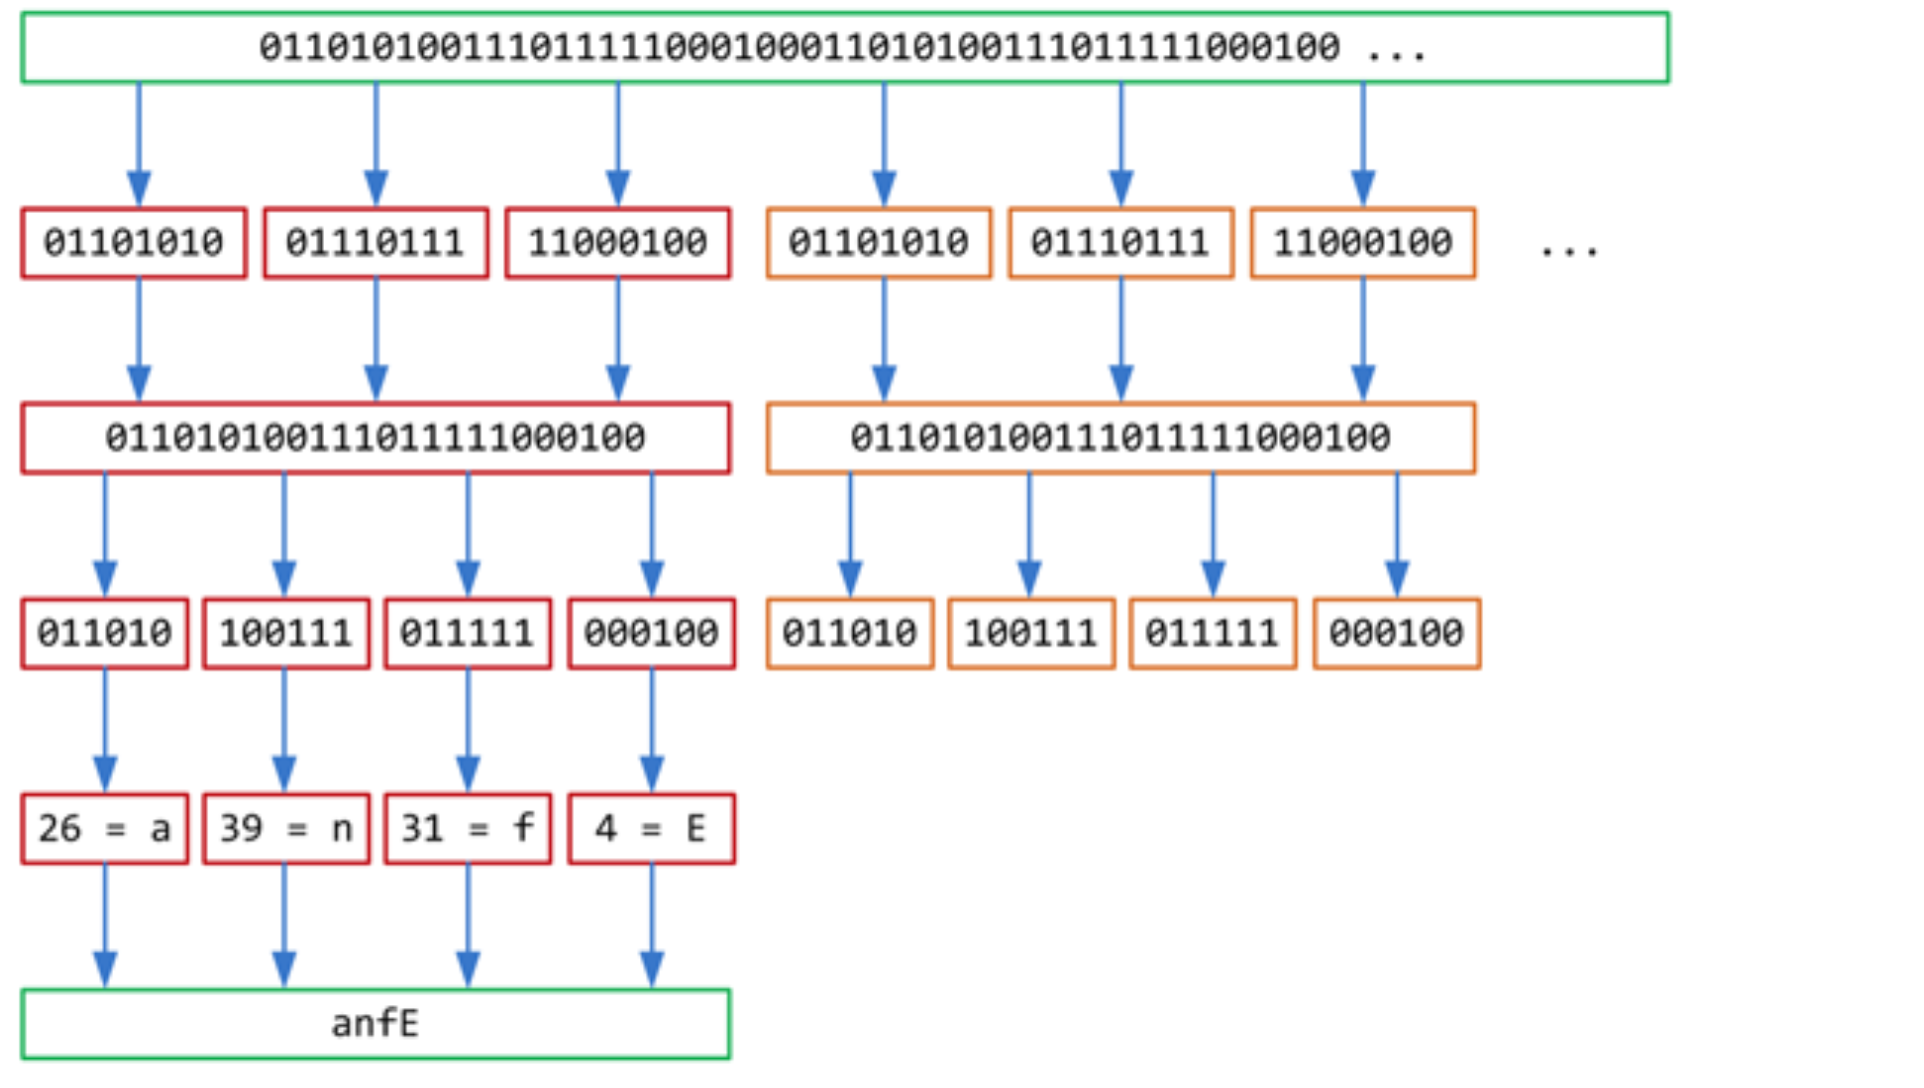
\includegraphics[width=\columnwidth]{b64}
    \caption{Subsequent conversion of binary data to bytes, bit sextets, and encoded characters \cite{App}.}
    \label{fig:b64}
\end{figure}

A first possible strategy is to apply simple data type casting, see List. \ref{lst:typecasting}.

\begin{lstlisting}[language=C, caption=Segmentation approach via type casting with pointers, label=lst:typecasting]
FLT floats[4] = {1, 2, 3, 4}
//actual array is of variable size;
CHR *bytes = (CHR *) floats;
\end{lstlisting}

The \lstinline{CHR* bytes} array could then be passed on to the encoding function. Test showed that this strategy seems to only work if the array to type cast does not contain any data before type casting. Thus, this approach is not appropriate here.

\bigbreak
A second possible strategy is to declare a \lstinline{union}, see List. \ref{lst:union}.

\begin{lstlisting}[language=C, caption=Segmentation approach via a union, label=lst:union]
union INTToCHR {
  INS i;
  CHR *c[sizeof(INS)];};
\end{lstlisting}

Here, both \lstinline[language=C]{i} and \lstinline[language=C]{c} refer to the same location in memory. This approach potentially works for a single \lstinline[language=C]{float}. As the \lstinline[language=C]{CHR*} arrays would need to be concatenated dynamically, this approach is (according to the author's opinion) not appropriate either. Test which were carried out using this strategy showed inconsistent outputs, indicating that the prompted data may not be contiguously stored.

\bigbreak
A third strategy for dividing the data arrays into bytes uses a combination of \lstinline[language=C]{malloc} and \lstinline[language=C]{memcpy}.

\begin{lstlisting}[language=C, caption=Segmentation approach via memcpy, label=mallocandmemcpy]
CHR *bytes;
bytes = malloc(header);
memcpy(&bytes[0], cf, header);
\end{lstlisting}

Testing confirmed that this method is successful. The \lstinline[language=C]{byte} array now contains the floats in contiguous order in binary form, stored as bytes. 

\bigbreak
The prepared data is passed to the base 64 encoding function \lstinline[language=C]{b64enc} in file \lstinline[language=C]{Yod.c}. The function takes some \lstinline[language=C]{CHR*} array \lstinline[language=C]{src} of length \lstinline[language=C]{len} as input, encodes it byte for byte and outputs character for character into the \texttt{VTK} output file \lstinline[language=C]{fout}. 

\bigbreak
The core of the algorithm (List. \ref{lst:b64alg}) was adopted from Malinen \cite{Mal05}.

\begin{lstlisting}[language=C, caption=b64 algorithm, label=lst:b64alg]
while (end - in > 2){
  putc(enc[in[0] >> 2], fout);
  putc(enc[((in[0] & 0x03) << 4) | (in[1] >> 4)], fout);
  putc(enc[((in[1] & 0x0f) << 2) | (in[2] >> 6)], fout);
  putc(enc[in[2] & 0x3f], fout);
  in += 3;}
  
if (end - in){
  putc(enc[in[0] >> 2], fout);
  if (end - in == 1){
    putc(enc[(in[0] & 0x03) << 4], fout);
    putc('=', fout);}
  else{
    putc(enc[((in[0] & 0x03) << 4) | (in[1] >> 4)], fout);
    putc(enc[(in[1] & 0x0f) << 2], fout);}
  putc('=', fout);}
return;}
\end{lstlisting}

In List. \ref{lst:b64alg}, \lstinline{in} and \lstinline{end} are \lstinline{CHR*} pointers which point to the beginning and end of the input array. Converting to base 64 requires rearranging the input in chunks of 6 bits. Each of these 6-bit chunks produces a value $\varv < 64 = 0b1000000$ and is able to be converted to one of 64 unique characters from the encoding array \lstinline{CHR* enc = "ABCDEFGHIJKLMNOPQRSTUVWXYZabcdefghijklmnopqrstuvwxyz0123456789+/"}. 

\bigbreak
For every $3$ bytes (or $24$ bits), the algorithm produces $4$ groups of $6$ bits, i.e. $4$ characters. The bits are extracted continuously via bit shifting. As mentioned before, the position or significance of the bits in the byte must not be violated. In other words, the value of the bit must not get lost through bit shifting. The algorithm is now explained in detail: 

\bigbreak
In line $2$, the first $6$ bits of the current character \lstinline{in[0]} are extracted by bit shifting to produce the first $6$-bit chunk. The value of this chunk is used to produce the index of the corresponding character in the encoding array \lstinline{enc}. 

\bigbreak
The last two remaining bits of the current input character \lstinline{in[0]} are evaluated and bit shifted in line $3$ to account for the first $2$ significant bits of the next $6$-bit chunk. The $4$ missing bits to complete the $6$ bits are extracted from the first $4$ bits of the second character \lstinline{in[1]}, again by bit shifting.    

\bigbreak
In line $4$, the $4$ remaining bits from the second input character \lstinline{in[1]} make up the first four bits of the next $6$-bit chunk. The missing $2$ bits of the $6$-bit chunk are extracted from the third input character \lstinline{in[2]}. This leaves $6$ bits of the third input character remaining, making up another $6$-bit chunk, as implemented in line $5$.

\bigbreak
If the input array length \lstinline{len} = \lstinline{end} - \lstinline{in} is not divisible by $3$, padding characters are required. The amount of padding padding depends on the amount of remaining input byes to complete a group of three input bytes. If $\rm{len}\,\%\,3==1$, two padding characters '==' are appended to the encoded string. If $\rm{len}\,\%\,3==2$, one padding character '=' is required. The algorithm is given in List. \ref{lst:b64alg}, lines 8-17.